1\documentclass{article}

\usepackage{multicol}
\usepackage[a4paper, margin=70px]{geometry}
\usepackage{hyperref}
\usepackage{graphicx}
\usepackage{geometry}
\usepackage{amsmath}
\usepackage{float}
\usepackage{xcolor}
\usepackage{cite}
\usepackage[numbers]{natbib}
%\usepackage[nottoc]{tocbibind}

\setlength{\columnsep}{1cm}

\title{ENME403 Report}
\author{Toby Bourke}
\date{May 2021}

\begin{document}

\begin{titlepage}
   \begin{center}
       \vspace*{1cm}

       {\huge\textbf{Final Year Project Progress Report E14}}
       \vspace{4cm}
		
		\textbf{Academic Supervisor: Shayne Crimp}\\
		
		\vspace{5cm}
		\textbf{Student Name: Toby Bourke}\\
		
		\textbf{Student ID: 84984154}\\
		
		\textbf{Student Email: tfb20@uclive.ac.nz}\\
		
       \vspace{1.5cm}
            
       \vspace{7cm}
       
       30\textsuperscript{th} of May 2021
            
   \end{center}
\end{titlepage}

\section*{Executive Summary}
% Why is this project important?
The purpose of this project is to produce a piece of software that can improve the well-being, productivity, and the ergonomics in primarily office environments. This will be achieved by creating software that works in conjunction of existing systems to generate a 3D map of the environment. This system is based on set of devices called Limpets that are attached to desks within an office environment.\\


% Who is this project for?
The project is for a company called Wellnomics. Wellnomics produces software for other companies that improve the well-being of employees and the ergonomics in the environment they work. Wellnomics has developed a new product that is used to gather more information about employees to further improve their developed software. The new product is the Limpets, and they can collect data of temperature, noise, etc. To work alongside the collected data, Wellnomics wants the Limpets to be able to find their location within an office environment relative to other Limpets.\\
% What are the user requirements?

The Limpets are required to be simple devices that do not need significant upkeep. Limpets are powered from a battery, therefore the Limpets require a minimal power consumption to maximise battery life. The Limpets need to be cheap and incredibly accessible, therefore the best method for generating a 3D map of all Limpets in an environment is using distance measurements through sound. Limpets use similar microphones and speakers to what phones use.\\

% What are the achievements so far? How much work has been done?
The current state of the project is, a method for generating a 3D map has been found, Audio Tone start detection has been implemented, a method of distance measurements with Limpets has been designed, and a system for multi-device syncing has been designed.\\

3D map generation is the creation of a 3D map of all Limpets within a network. Audio Tone start detection is used to find when an incoming tones starts, this is used by a distance measurement system to get accurate distance measurements. A distance measurement method has been developed as most systems rely on reflecting sound off an object and recording how long the round trip took to take a measurement. Due to limitations of the Limpets, they cannot use the same method of distance measurement as other existing implementations. The multi-device syncing system has been designed to allow a large network of Limpets to work together to complete all distance measurements required to generate the 3D map.\\

%What will be worked on to complete this project
Further work is required to complete this project. This work is the implementation of the distance measurement system, implementation of multi-device syncing, and 3D map generation. Each of these steps require the previous to be completed. Distance measurement is a two step process of having successful distance measurements with external hardware, then using Limpets to achieve a distance measurement.


\pagebreak
\tableofcontents
\pagebreak

\section{Project Overview}
\subsection{Project Objective and Justification}
				%Why is the project being undertaken?
The purpose of the project is to develop software that improves the well-being of employees and the ergonomics of primarily office spaces. This project is for a company named Wellnomics. Wellnomics is a company that develops systems to improve the health, well-being and productivity of computer users at companies. Wellnomics primarily produces software, and this project is their first attempt at making a physical product.\\ 

The developed software will take the form of an indoor mapping system using distance measurements that produces a 3D Mesh. This system is required to work in conjunction with existing systems and their related hardware. The existing hardware is shown in Figure \ref{fig:limpet} and is called a Limpet. These Limpets only method accurate method of measuring distance is the use of a speaker and microphone.\\

\begin{figure}[H]
	\centering
	\noindent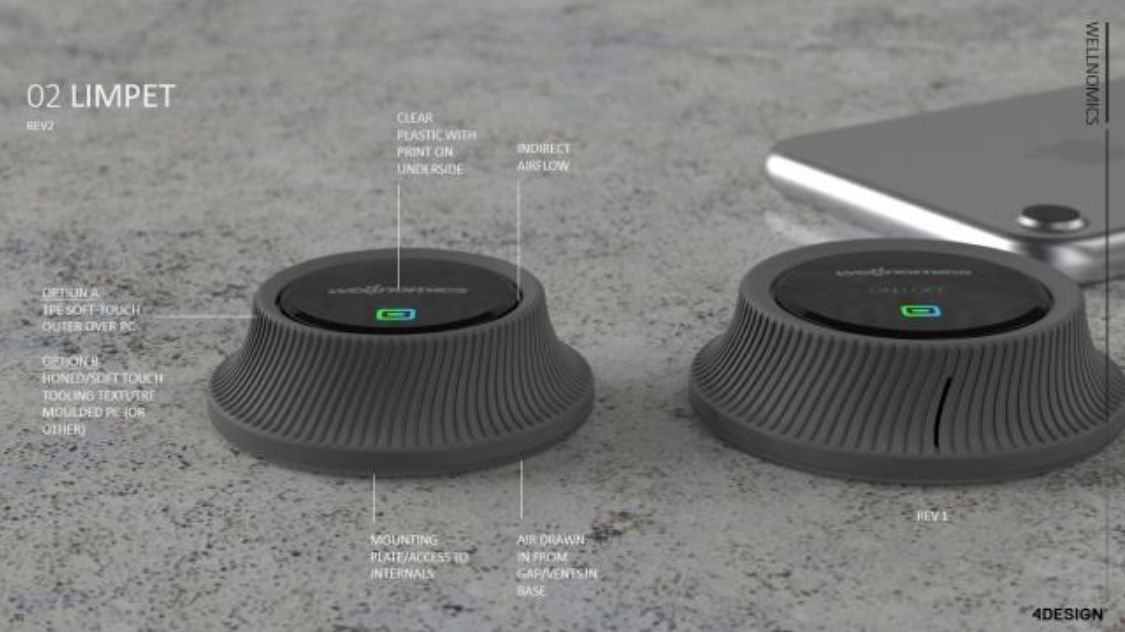
\includegraphics[width=0.5\textwidth]{images/limpet}
	\caption{Limpet Device}
	\label{fig:limpet}
\end{figure}

Limpets track information of an employee at any desk they are attached to. Examples of tracked information include but are not limited to, desk height, if the employee is actively typing or not.\\

The Limpets cause constraints on the solution to the problem. All implemented solutions require to have a low power consumption. The Limpets are only capable of using sound for accurate distance measurement. The sound can be produced by a 5V speaker and can be recorded using a MEMs microphone. The environment that the Limpets will be implemented into may have noise that needs to be accounted for to improve distance measurement accuracy and range. 3D Mesh generation is not required to be done on the Limpets, and can be done on a server or computer. The accuracy of the 3D Mesh needs to be within 90\% of reality, e.g. a one metre distance between two points needs to be within $\pm$10cm.\\ 

The indoor mapping system in a hot-desk office environment context would track the locations of desks throughout a building. The location information of desks can be used in conjunction with other information gathered through the limpets. With the combined information of desk location and gathered information, employee productivity and well-being can be tracked compared to desk location.\\

Knowing the location of employee productivity and well-being relative to key features within an office environment can be used by employers and companies to improve the working environment. For example, if employee well-being is increased near windows in an office building, the office might be rearranged to maximise the number desks near windows. This benefits both employees and the companies that hire these employees.\\

A successful solution to the project would be a software solution that generates a 3D Mesh of all locations of the Limpets within an office environment. The software solution would be required to handle any number of Limpets within a network, possibly thousands. This is all required to be done without breaching any constraints placed by Wellnomics.

\subsection{Work Identification}
The work for this project has been split across the team working on this project. The project was split into four individual parts, the speaker, the microphone, the audio transmission, and the software. The break down of these sections was to improve the overall expertise of the team as a whole as more time could be dedicated to understand only one part instead of all aspects of the project.\\

The speaker aspect of the project focuses on how the speaker produces sound, the attributes on the produced sounds, and how to drive the speaker. The result of this is a functional speaker module that can be used for testing distance measurements and 3D Mesh generation with system produced by the software aspect of the project.\\

The MEMs microphone member has to find all relevant information on how MEMs microphones work, how accurate the recorded sound is to reality, and how to interface and record sounds. This will be combined with the speaker module to produce a prototype Limpet capable of create and recording sounds.\\

The audio transmission aspect of the project focuses on how sound acts within a office environment, and the best method for generating sound to maximise the effective range of distance measurements. This aspect of the project require extensive research into what materials are within office environments and their effects on sound waves of varying frequencies. The results of this would either the best frequency to use for distance measurement or the best approach to deciding the best frequency to use for distance measurement.\\

The software aspect of the project focuses on connecting all other aspects of the project together. The software will take the recorded sound from the MEMs microphone of the speaker making a tone and calculate a distance measurement. Once all Limpets in a network have had measurements taken, these distance measurements would be used to generate a 3D Mesh.

%-----------------------------------------------------------------------------------------
\pagebreak
\section{Progress to Date}
This section covers progress completed to date by Toby Bourke.
\subsection{Background Research}
%Taking distances between objects and converting them into a mesh
\subsubsection{3D Mesh Generation}
One of the final steps in the project is creating a 3-Dimensional mesh of all limpets in a network. Due to limitations of the measurements capable of being taken by the limpets, only the distance between limpets can be found and not orientation. This limitation meant that generating a 3D mesh of the limpet network wasn't a simple task.\\

Before doing research, the problems with only distance measurements and no direction were shown as to justify doing research. This was done by initially taking N points and seeing if arbitrary distances between all points can construct only one possible mesh with one know point.\\

Figure \ref{fig:3PMesh} shows the only possible combination for a 3 point mesh, with one originally known point. Figure \ref{fig:4PMesh} shows that there are at least two possible combinations, with one originally known point. As there is more than one possible combination for a four point mesh, research needs to be done into possible ways of generating a mesh of N points that is accurate to the real positions of the limpets relative to each other.\\

\begin{figure}[H]
	\centering
	\noindent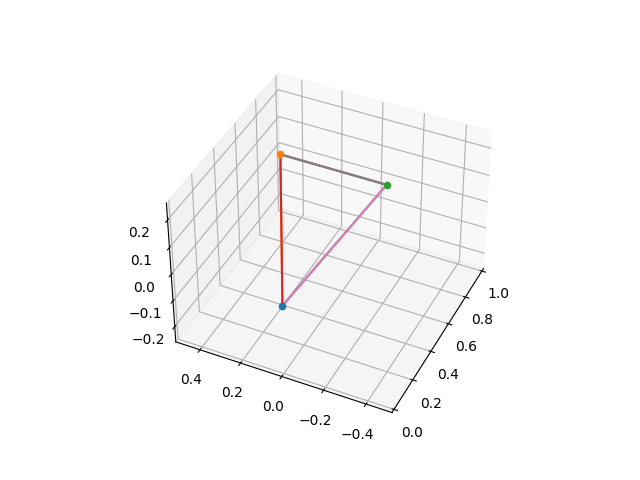
\includegraphics[width=0.49\textwidth]{images/3LimpetNet}
	\caption{Three Limpet Mesh Possible Configurations}
	\label{fig:3PMesh}
\end{figure}

\begin{figure}[H]
	\centering
	\noindent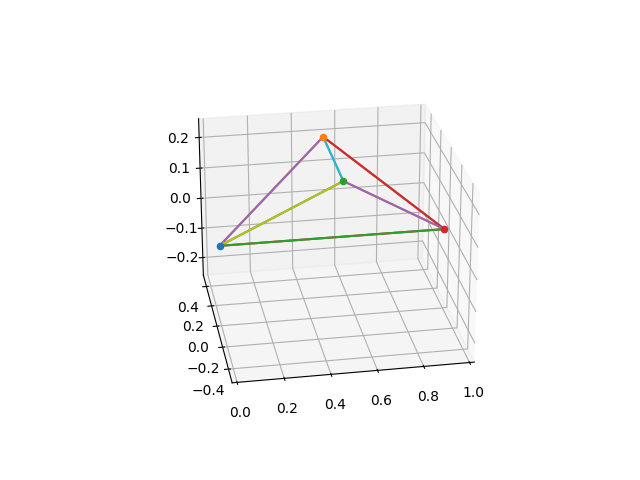
\includegraphics[width=0.49\textwidth]{images/4LimpetNet}
	\noindent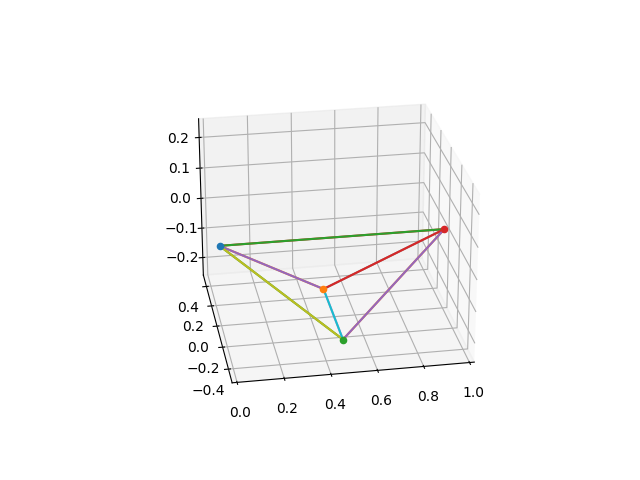
\includegraphics[width=0.49\textwidth]{images/4LimpetNetFlip}
	\caption{Four Limpet Mesh Possible Configurations}
	\label{fig:4PMesh}
\end{figure}

While researching, an existing system was discovered that found the location of an object based only on distance measurements between objects. The existing system was GPS Satellite Tracking. GPS uses four satellites which position are known relative to each other to find a fifth point with unknown location \cite{gps}. The same system which GPS uses with four known points to find the relative location of a unknown point can be implemented to generate a mesh.\\

%Methods to display the mesh in a visually meaningful way ????

%Methods of detecting when a tone starts
\subsubsection{Audio Tone Start Detection}
Detection of when a tone starts is a very important feature when trying to accurately measure distance. If the start of the tone is not accurately measured the measured travel time of the tone will not be accurate.\\

Ultrasonic distance sensors already use sound to measure distance. Ultrasonic sensor use minimal processing to produce a distance measurement as it is assumed that if the emitted tone is picked up at any point, it will be accurate enough \cite{toa_akeem_2020}. This approach was proven to cause significant inaccuracy when working within the audible range of frequencies.\\

Within the music industry detecting the start of notes of music instruments is a common problem, the algorithms used are called Audio Onset detection algorithms. There are many approaches for doing audio onset detection from thresholding to machine learning \cite{bock2012evaluating}.\\

\subsection{Theoretical Designs}
% Measuring Distances between objects that can take time to process (virtual walls)
\subsubsection{Distance Measurement}
Measuring distance between two points using sound requires recording how long a sound takes to travel between the points. Ultrasonic distance sensors do this by sending out a tone that bounces back off an object and records how long it took the sound to travel the round trip, this time is halved to get a one-way trip period. The one-way trip period is then used to calculate the distance based off the speed of sound.\\

The limpet's cannot physically bounce a sound off of another limpet as the limpets cannot control the direction of emitted sound. This limitation means that the limpets cannot individually measure the distance between themselves and other limpets.\\

The first approach to measuring distance is to use the inbuilt Real Time Clock (RTC) of the controller within the limpet. In a system of two limpets, one limpet would be programmed to emit a sound at a specific time and the other limpet would start recording how long it has been since a sound was emitted. Figure \ref{fig:limpetOneway} is a visualisation of how the one way communication works.\\

\begin{figure}[H]
	\centering
	\noindent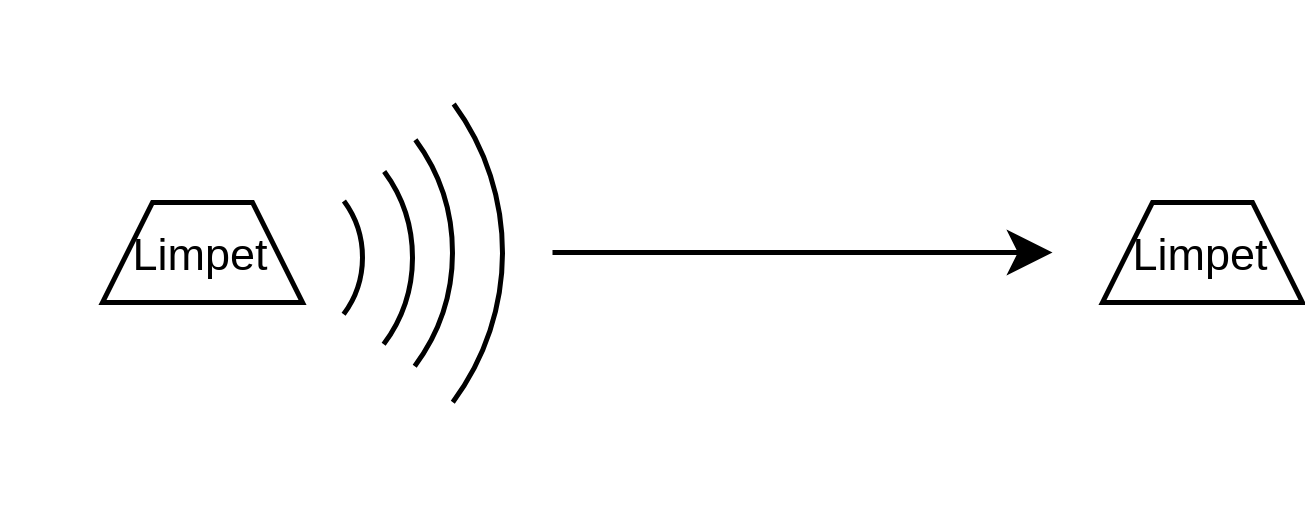
\includegraphics[width=0.71\textwidth]{images/limpetOneway}
	\caption{Limpet One-way Distance Measurement}
	\label{fig:limpetOneway}
\end{figure}

The one-way distance measurement relies on the RTC being accurate over long periods \cite{rtccomp}, from days to months, as a one meter difference in the distance measurement can be induced with a 3 millisecond difference between the RTC clocks. The RTC clock within the Nordic nRF52840 used in the limpets has a clock accuracy of $\pm$500ppm \cite{nrf52840}. The 500ppm results in a maximum shift in the RTC of ~$\pm$42 seconds in a day. 42 seconds equates to a measurement of distance incorrect by 13.9km, well beyond the acceptable error.\\

As can be seen the one-way distance measurement is not a suitable solution to the problem. The second approach that was designed was creating a virtual wall that bounces a sound between the limpets. This is achieved by when receiving a tone, a response is produced. The time between sending and receiving the time could then be used to calculate the distance without the need for reliable clocks over long periods. Figure \ref{fig:limpetTwoway} shows the process, step 1 send message, step 2 process message, step 3 send response.\\

\begin{figure}[H]
	\centering
	\noindent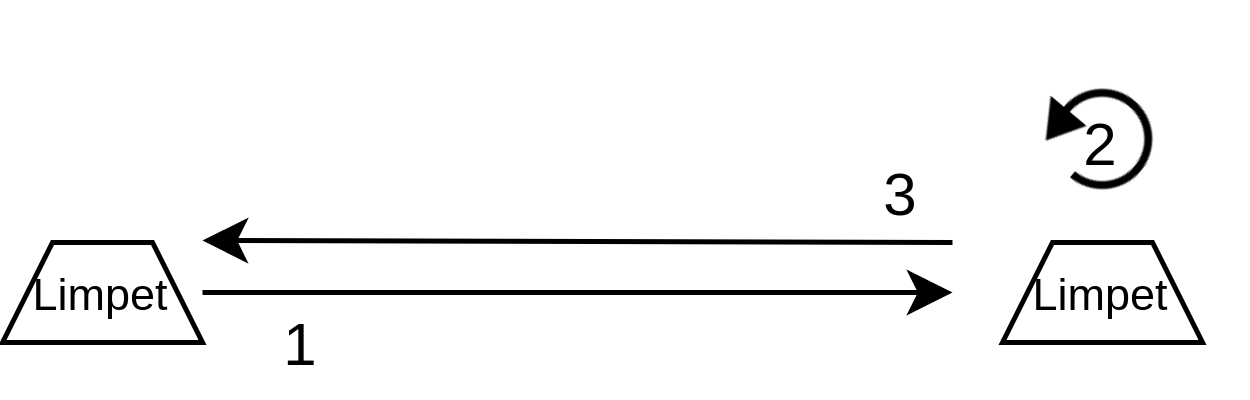
\includegraphics[width=0.71\textwidth]{images/limpetTwoway}
	\caption{Limpet Two-way Distance Measurement}
	\label{fig:limpetTwoway}
\end{figure}

The two-way distance measurement works if the processing for each limpet is know, this is possible to artificially increase processing to guarantee known periods. The known processing time can be subtracted from the time between sending and receiving. With the known two-way trip period the distance between the two limpets can be calculated. This provides a distance measurement between the two limpets to the limpet that started the measurement.\\

The two-way distance measurement can be improved upon by making it a 3-way measurement that provides a distance measurement for both limpets. Figure \ref{fig:limpetThreeway} shows the implementation of how the limpets would send messages.

\begin{figure}[H]
	\centering
	\noindent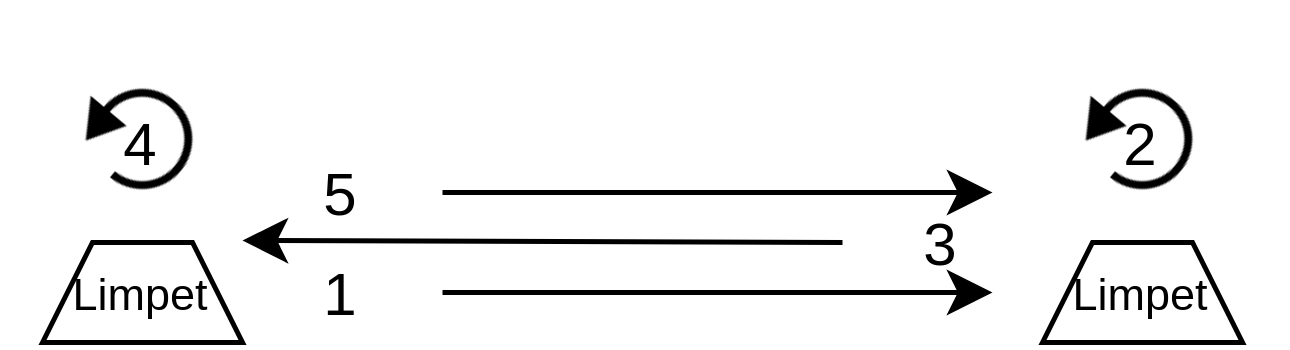
\includegraphics[width=0.71\textwidth]{images/limpetThreeway}
	\caption{Limpet Three-way Distance Measurement}
	\label{fig:limpetThreeway}
\end{figure}

% Mesh system communication for sequencing
\subsubsection{Multi-device Syncing}
A full network of Limpets could be in the the hundreds, as a consequence when a measurement is to be taken multiple Limpets could try to talk over each other. To remedy this an order of operations was constructed that decided on which Limpet was talking, and how the Limpet talked to others. This order is as follows:

\begin{itemize}
\item Initialise Decider
\item Identify Nearby
\item Distance Measurements
\item Information Distribution
\end{itemize}

A visual representation of the process can be seen in Figure \ref{fig:limpetHeirachy}.

\begin{figure}[H]
	\centering
	\noindent\includegraphics[width=0.71\textwidth]{images/limpetHeirachy}
	\caption{Limpet Multi-device Distance Measurement Process}
	\label{fig:limpetHeirachy}
\end{figure}

Figure \ref{fig:limpetHeirachy} Step 1 is the Initialising Decider operation. Initialising Decider is an operation that decides which Limpet should start making distance measurements. This could be decided based on the limpet with the lowest ID for example.\\

Step 2 is the Identify Nearby operation. Identify Nearby is an operation that identifies all nearby limpets that could possible hear it's distance measurement. This can be done through using the Limpets onboard Bluetooth capabilities or through the speaker and microphone.\\

Distance Measurements is an operation where the initial Limpet tells a device it is going to measure the distance between them. This is repeated until all Limpets that were identified have had the distances measured.\\

Information Distribution is an operation where all gathered distance measurements are provided to neighbouring Limpets as maximise the chance that distance measurements between Limpets are uploaded to a server. This operation also decides the next Limpet that will gather distance measurements, repeating the process.\\
\subsection{Software Development}
% Development of detecting start edge
A core feature of measuring distance is accurately measuring when a sound is received. Ultrasonic distance sensors use when a peak is detected \cite{toa_akeem_2020}, to see if the same approach is possible a script was created. The object of the script was record sound, and then detect the starting point of a tone that is played during the recording.\\

Figure \ref{fig:pulse500} shows three graphs produced by a recording with a 500Hz tone being played. The top graph is a Fast Fourier Transform (FFT) of the entire recording period. The middle graph shows in blue the raw input audio signal and in orange is the raw input audio signal with a band-pass filter at 500Hz applied. The bottom graph is the dB of the band-pass filtered signal, this isn't scaled accurately but the dB differences is correct.

\begin{figure}[H]
	\centering
	\noindent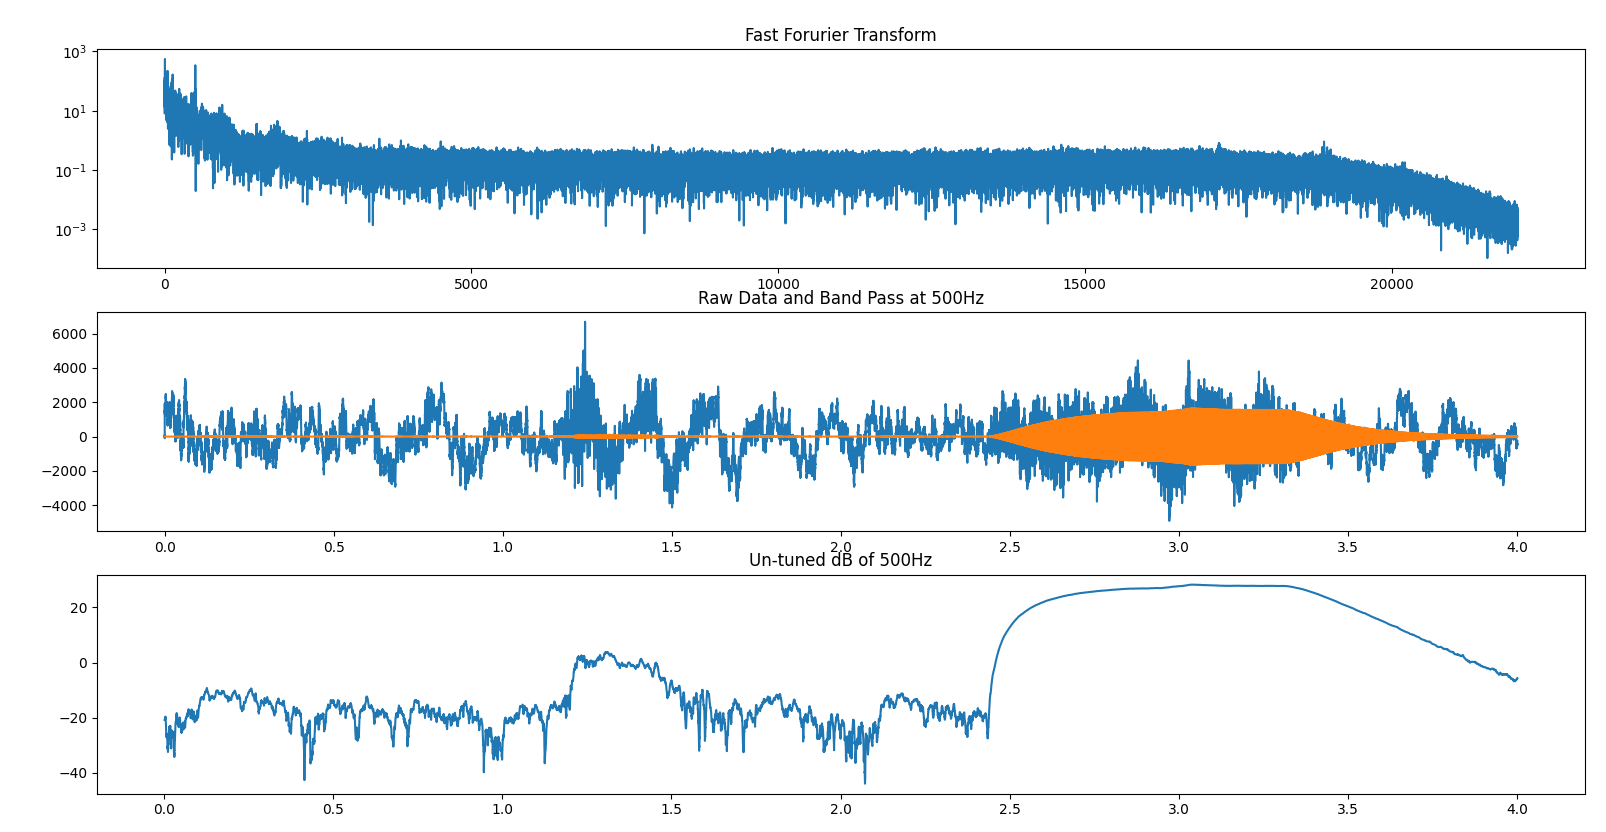
\includegraphics[width=0.9\textwidth]{images/Pulse500Hz}
	\caption{Audio Received and Processed for Incoming 500Hz Tone}
	\label{fig:pulse500}
\end{figure}

Figure \ref{fig:pulse500} shows that the 500Hz sound doesn't increase in amplitude quickly. As a result of this slow rise is if a threshold was used like in ultrasonic distance sensor, the point at which the tone is detected would be out by multiple milliseconds. This inaccuracy is unacceptable as it would translate to metres of error.\\

To improve accuracy, different Audio Onset detection algorithms were used. All implementations of more complicated techniques like overlapping the input signal over an expected waveform, and example of which is shown in Figure \ref{fig:shapeOverlay}, had a significant flaw. The more complicated algorithms processing time was significant, as most Audio Onset algorithms weren't designed with real time embedded systems in mind.

\begin{figure}[H]
	\centering
	\noindent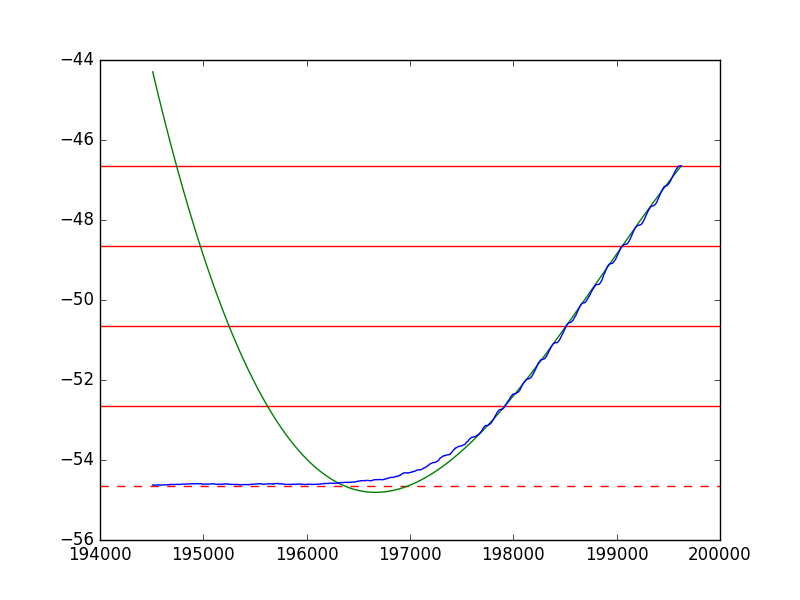
\includegraphics[width=0.5\textwidth]{images/signalShapeOverlay}
	\caption{Overlaying a Curve on Data to find Audio Onset}
	\label{fig:shapeOverlay}
\end{figure}

The most effective solution that was implemented was first finding the tone, currently using a threshold, and then using the current gradient of the input data. The script would follow the slope until the gradient changed from sloping up to being level or sloping down. Figure \ref{fig:gradient} shows the method being implemented. First the input signal has a band-pass filter applied, then the envelope of the signal is taken, the blue line on the bottom graph. Using a threshold to find any point of the incoming tone, a a gradient is found at that point. The the data is stepped through going backwards through time until the gradient is no longer indicating an upwards slope.

\begin{figure}[H]
	\centering
	\noindent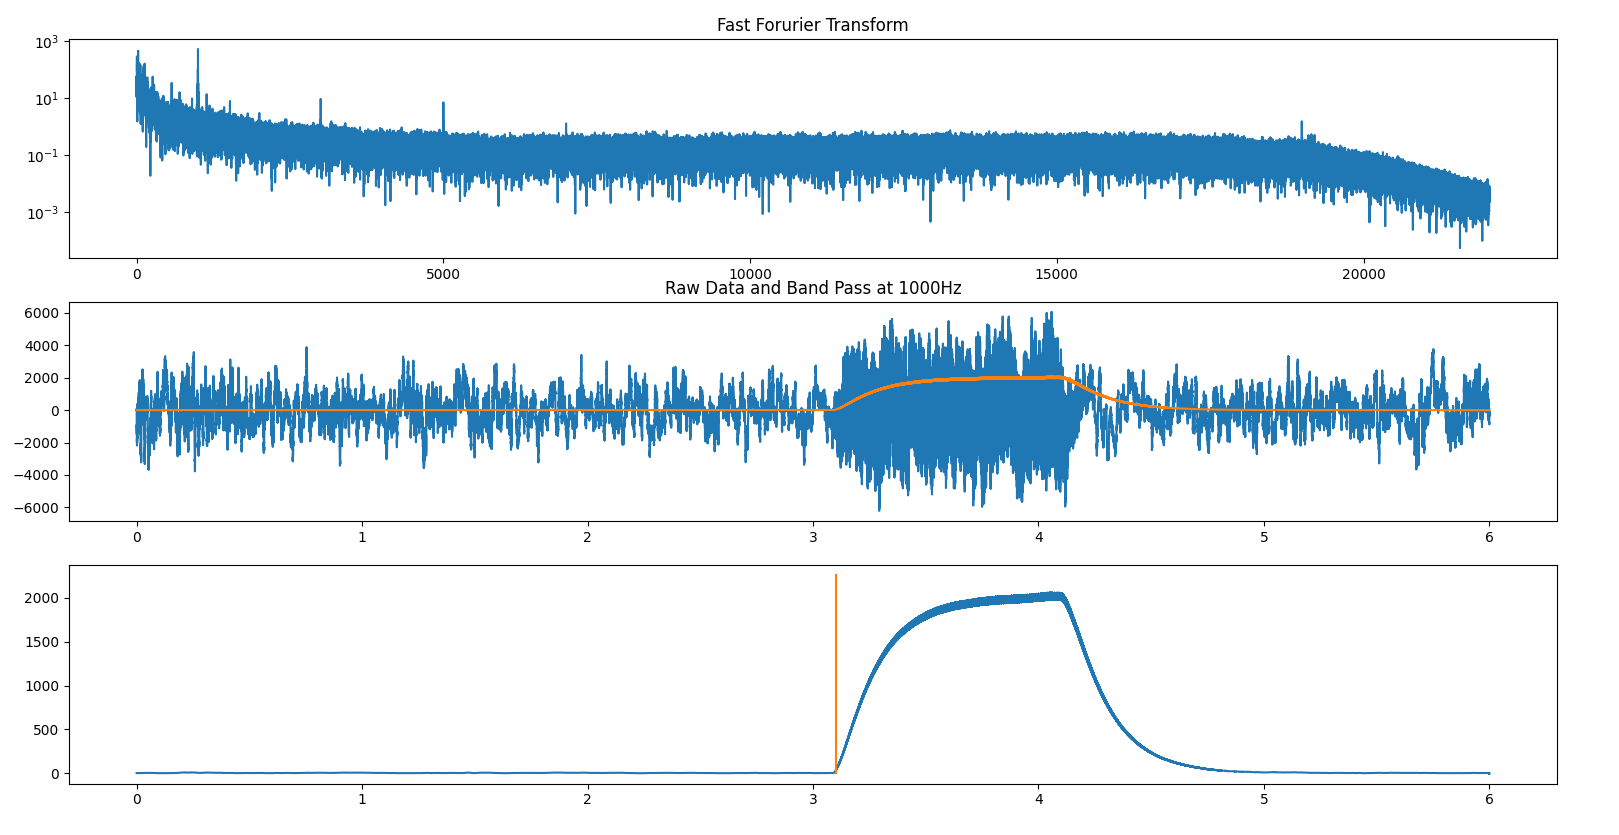
\includegraphics[width=0.9\textwidth]{images/gradientDetection}
	\caption{Start of Tone Detection Using Gradient}
	\label{fig:gradient}
\end{figure}

This solution though effective, does not always work. The generated tone can not be detected in some cases, e.g. inconsistent volume of the tone. Further improvements and tuning is required to improve Audio Onset detection. 

\subsection{Summary and Conclusion}
A completed prototype for testing has not yet been completed. The speaker and driver circuit has been successfully implemented and can used for further testing. The MEMs microphone has not successfully been interfaced with as such an alternative is being used until the microphone can be correctly setup.\\

Research into all how sound responds in an office environment is currently on going. Current research indicates that the entire functional range of the speaker is likely equally capable of conducting distance measurements.\\

The current research and theoretical designs of 3D Mesh generation, distance measurements, and multi-device syncing all currently cannot be implemented. Implementation of these system requires further development of a prototype Limpet. The method of Audio Onset detection has been successful at detecting the beginning of tones, though may still require further tuning and development to increase accuracy.



%---------------------------------------------------------------------------------------
\pagebreak
\section{Remaining Tasks}
\subsection{Tasks}
The remaining tasks that need to be completed are as follows:

\begin{itemize}
\item Distance Measurement
\item Prototype Distance Measurement
\item Multi-device Syncing
\item 3D Mesh Generation
\end{itemize}

\subsubsection{Distance Measurement}
The implementation of measuring physical distances is the next steps. To achieve this the prototype speaker controller and Audio Onset detection algorithm will be used in combination with a computer to measure a distance.
\subsubsection{Prototype Distance Measurement}
After distance measurements have been successfully implemented, completing distance measurements onboard a microcontroller is the next step. This step will be completed by using an completed prototype device that has both functional speaker and microphone.
\subsubsection{Multi-device Syncing}
When distance measurements can be taken between two prototypes, the next step is to attempt to take measurements between multiple devices with coordination. This will entail implementing and testing the Multi-device Syncing algorithm that has been developed.
\subsubsection{3D Mesh Generation}
Once distances can be measured throughout an entire network, this network of distances then needs to be converted into a useful form. A 3D mesh of all the Limpets in the network will be constructed using the same method as the researched GPS tracking method. This 3D mesh generation is not required to be done on a Limpet.

\subsection{Timeline}
Figure \ref{fig:gantt} is an updated Gantt chart that shows the plan for the entire project. Currently the testing stage should have started, though this has not yet happened.
\begin{figure}[H]
	\centering
	\noindent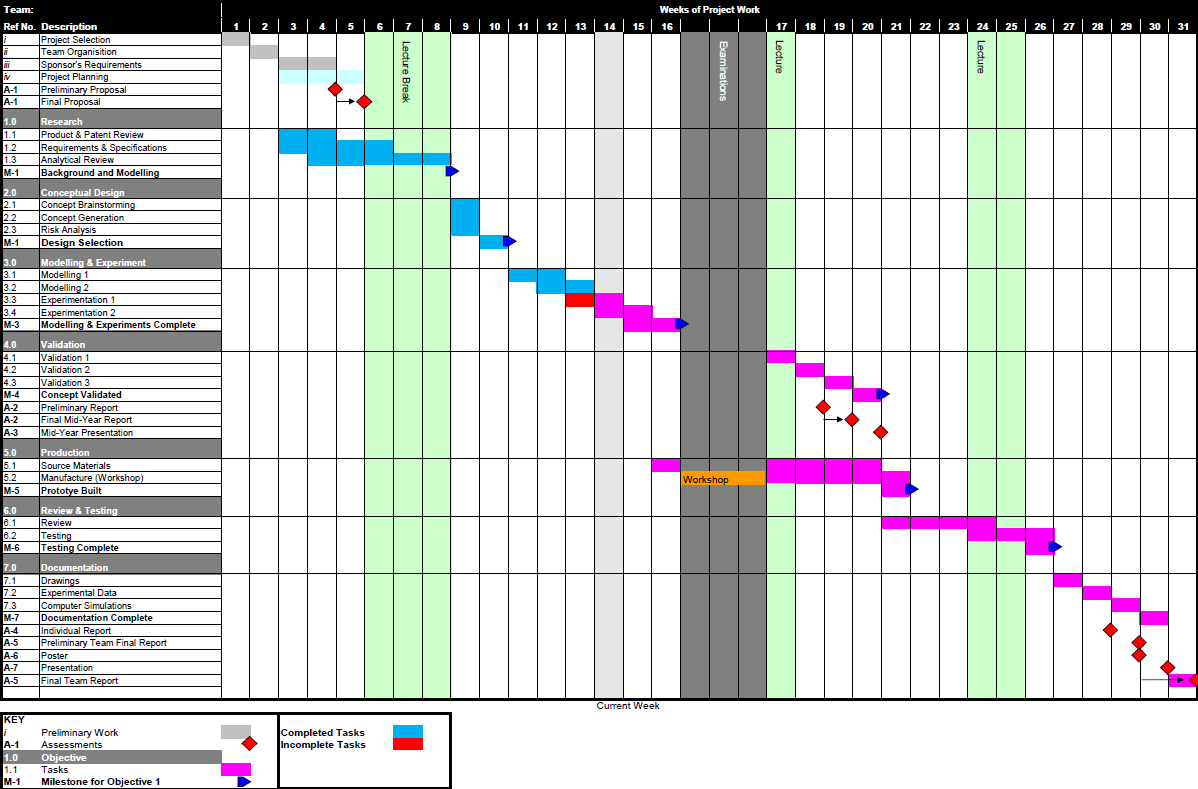
\includegraphics[width=\textwidth]{images/gantt}
	\caption{Gantt Chart for Timeline}
	\label{fig:gantt}
\end{figure}
\subsection{Budget Summary}

The current expenses of the project is shown in Table \ref{tab:budget}. There should be no additions to this budget until after system testing has begun.

\begin{center}
	\begin{table} [H]
	\centering
		\caption{Budget Summary for Project}
		\begin{tabular}{|c |c c c|}
			\hline
			Item & Cost & Qty & Total Cost (NZD)\\
			\hline\hline
			Teensy 4.0 & \$32.17 & 4 & \$128.68\\
			MEMs Microphone Developer Board & \$12.25 & 5 & \$61.25\\
			Class D Amplifier (XC4448) & \$5 & 2 & \$10\\
			\hline\hline
			Total Cost & &  & \$199.93\\
			\hline
		\end{tabular}

		\label{tab:budget}
	\end{table}
\end{center}

% Actual distance measurement
% Implementation of accurate distance measurement onto micro controller
% Implementation of Multi-device syncing
% Implementation of 3D mesh generation from distance measurements

\pagebreak
\section{Sustainability Analysis - Life Cycle Analysis}
\subsection{Base Component Procurement}
\subsubsection{Silicon Semiconductors}
Silicon is mined as quartz ($SiO_2$), it is refined into a metallurgical state. The metallurgical state is refined a further three times, this produces a 99.9999\% pure silicon wafer. Each step requires resources for production and results in wasted silicon. Processing silica to a wafer requires 2100kWh/kg of energy \cite{siliconLCA}. The total amount of carbon emissions as a result is dependent on regional factors for how the energy is produced.

\subsubsection{Battery}
Lithium batteries are common batteries for use with portable electronics. The battery cell is constructed out of five components: the anode, cathode, separator, electrolyte and cell container \cite{BATTLCA_1}. Each component of the battery require energy to produce, and as such pollution produced by the components manufacturing is primarily dictated by local energy production.
\subsubsection{Housing}
It is assumed the housing is constructed using a 3D printer with polylactic acid or PLA. PLA is made from fermented plant starch such as corn, sugar cane etc. The growth of these plants requires land preparation, maintenance and harvesting which all have impacts on the environment be through energy usage or chemicals. For sugarcane grown PLA, the total $CO_2$ emissions from growth to PLA production is 501kg/ton PLA \cite{PLALCA_1}. PLA plastic produces less $CO_2$ emissions than other types of 3D printer materials when looking at the transportation \cite{PLALCA_2}.

\subsection{Production}
The manufacturing of the Limpets' housing being through the use of 3D printing with PLA means there is little environmental effect. The primary source of environmental effects with 3D printing come from the use of energy to run the printer \cite{3dprint}.\\

Through the use of the correct methods, the environmental effects of PCB manufacturing can be improved. The use of more environmentally friendly materials, and resins can decrease the harmful effects on the environment \citep{esfandyari2015lean}. There is limited improvements that can be made to the PCB assembly process as this step of the process primarily only requires energy. The environmental effects are dictated by how energy is produced where the PCB is being assembled.
%PCB Manufacture
%	Carbon emissions, toxicity of production, waste

\subsection{Distribution}
%Shipping
%	Shipping with desks
%	Shipping without desks
%Setup
%	Labour
%	Instillation costs
Limpets can be sold individually or attached to desks, meaning that they can be shipped in different forms. The primary method of distribution is freight on ships due to the size of desks and quantity of limpets that would be used by each user. Freight ships have a large range of environmental impacts, for example, air pollution, spills from ships, ship-strikes on marine megafauna, and ballast water containing aquatic invasive species \cite{WALKER2019505}.\\

Limpets that have been attached to desks have to be shipped at least twice before they arrive with a customer. This double shipping comes from the limpet being shipped to desk distributors to attach the limpets then the desk distributor shipping the desks. The installation process has related costs as it require labour to complete the installation, though this cost is limited as the installation process is simple.\\

Limpets sold individually from desks have less related shipping costs as they will go directly from Wellnomics to customers. The installation costs for the customer is larger than if they came preinstalled with the desks as each limpet require to be manually installed either by a user or qualified worker. The costs incurred would not be significant as the installation process is designed to be simple.

\subsection{Usage}
The usage phase of a Limpet's life-cycle is where the devices are in use in offices. The Limpets have both operational requirements and maintenance requirements.\\

A major operational requirement of the Limpet is energy. Energy for the Limpet comes in the form of a Lithium coin-cell battery. The operational lifespan of a coin-cell Lithium battery is three years \cite{liioncoincell}. The use of a battery instead of external energy source means during operation the Limpet has no effect on the environment. Due the battery requiring being charged or replaced, not being powered externally means there will be required maintenance of the devices. Features that Limpets provide mean that improvements of energy use can be implemented, reducing overall energy use even with increased use from the Limpets.\\

In the case of a Limpet requiring repairs, the device would likely be replaced. This is due to the Limpets being a low cost device, and incurred costs of repairing a Limpet may be more than the Limpet is worth.\\

\subsection{End of Life}
At end of life iof the limpets, the batteries are removed and are shipped to a battery recycling facility. The battery recycling facility removes all non-metal parts and ships the leftover mixed metal to a metal separation facility \cite{batteryuni}. The PCB of the limpets can be recycled in three ways, thermal recovering, chemical recovering, and physical recovering \cite{candorInd}.\\

For the thermal recovering process, you must heat the PCB to a high temperature the remove the metals present on the board. PCBs are generally made from FR-4 that is a composite material composed of woven fibreglass cloth with an epoxy resin binder. Thermal recovery will incinerate the FR-4 but retain the copper. This method will produce harmful gases, these gasses can contain lead and dioxin for example.\\

For the chemical recovering process, a bed of acid is used to recover metal from the PCB. The board gets put into the acid, which destroys the FR-4. This process produces large quantities of wastewater that need to be handled and processed further.\\

The physical recovery process involves the shredding, smashing, breaking, and separating of the metal from non-metal components. While this method does have the least environmental impact,
it is a hazardous for workers. The process produces metal, and glass particles that are released into the air. Small particles can lead to respiratory issues if exposed for prolonged periods. This method does retain all the metal components.

% --------------------------------------------------------------------------------------
\pagebreak
\section{Conclusion}
%Overall Progress
The focus of this project is the creation of a complimentary system to a product Wellnomics is developing. This complimentary system is to improve the well-being and productivity of employees at a company where the Limpets have been implemented. The system is a mapping system that takes advantage of hardware on the Limpets Wellnomics has designed. Multiple system were researched, designed and/or implemented to achieve this goal. These systems are as follows, 3D Mesh generation, Audio Tone Start Detection, Distance Measurement, and Multi-device syncing.\\

The 3D Mesh generation system was researched to find an effective method of finding relative positions of Limpets to other Limpets within a network. The solution found is the same that is used within GPS systems, four points with known location finding the position of a fifth point with only distance measurements. This system has yet to be implemented, it will not be implemented until accurate distance measurement between a network of Limpets can be achieved.\\

Audio Tone Start Detection is a problem that is required to be solved as inaccurate measurement of when a tone starts can cause significant deviations in distance measurements. A recorded travel time being incorrect by 3ms will result in a ~1m deviation of the distance between Limpets. This required accuracy meant the simpler solution of using Ultrasonic distance sensors could not be used. The method being used is an Audio Onset algorithm that uses the gradient of an envelope of the incoming sound to find when a incoming tone starts.\\

The Audio Onset algorithm has been implemented. The solution does not work perfectly and requires further development to be more resilient to external noise. The current solution is capable of being used within controlled environments and can be used for further testing of systems.\\

Distance measurement is not a simple task, most systems that use sound to do distance measurement reflect sound off an object. The Limpets cannot direct sound towards specific direction so an alternative solution was developed. This solution is using Limpets as virtual walls, after receiving a sound the Limpet responds. This create a virtual wall which can be used by a Limpet to measure distance from different Limpets. This system can be expanded if the original Limpet responds to the second Limpets response, this allows the second Limpet to get a distance measurement between the two Limpets. This system has yet to be tested as the Audio Onset detection has just reached a functional form.\\

Multi-device Syncing is a process that has been designed to allow networks of more than two Limpets accurately measure distances. This has the steps, initialise decider, identify nearby, distance measurements, and information distribution. Initialise decider simply means deciding on which Limpet starts taking distance measurements. Identify nearby is the step where the currently active Limpet identifies other Limpets to do distance measurements with. Distance measurement has the Limpets do distance measurements to all nearby Limpets. Information distribution is the active Limpet providing it's neighbours with the distance measurements it has taken. This system has not yet been implemented, it requires distance measurements taken with prototypes first.\\

The life-cycle analysis of the Limpets indicate that there are negative effects on the environment from this device. These effects on the environment can significantly mitigated if the correct processes are taken at the end of life and green methods of energy generation are used in the production of the Limpets.


\pagebreak
\bibliographystyle{IEEEtran}
\bibliography{ref}

\end{document}